\documentclass{beamer}
%\usepackage[utf8]{inputenc}
\usepackage{amsmath}
\usepackage{graphicx}
\usepackage{url}
\usepackage{hyperref}

\title{Convergence of Divergent Series}
\date{}
\author{}

\begin{document}
%\pagenumbering{gobble}
\pagenumbering{arabic}
\maketitle
\tableofcontents
\listoffigures
\listoftables
\newpage

 \begin{center}
 "Divergent series are an invention of the devil and it is shameful
to base on them any demonstration whatsoever."\cite{Abel}
 \end{center}
 \begin{flushright}
   N.H. Abel. 1826
   \end{flushright}
%\section{Abstract}


\begin{abstract}
    Mathematics is the science of skilful operations, which are dealing with the logic of shape, quantity
and rearrangement. Mathematics is using its core principles and rules to solve problems and get a
reasonable answer. In my opinion, mathematics will soon run out of interesting theories if all new
theories will formulate in terms of invented concept, which appear in axioms. This exploration is
about finding finite values, limits for famous divergent series and later analytically extending
Euler-Riemann's zeta function to find a limit for any divergent series that can be formed by Euler-
Riemann's zeta function.
\end{abstract}

\section{Introduction}

\paragraph I tend to think that in order to create innovative theories, mathematics as a whole should be pushed
to its boundaries and limits, new axioms should be invented and unexplored topics should be studied.
With this kind of approach, I got acquainted with the divergent series. It all has started in my former
school when I was in 7 th grade and we have started the topic of geometric series. When my
vteacher asked a question – "What will be the infinite sum of one, a half, a quarter and so on?"
Initially, I thought the answer was infinity, because at that time it made sense to me, an infinite
amount of values equals to always growing sum until it reaches infinity. When the teacher told us
the answer is two, I was quite shocked by the fact that it has an end and all these values are
converging to one finite value. I remember how I was walking around and trying to understand,
why this series does not go beyond that finite value? It was logical to me that if it keeps summing
every element, every element should contribute to the goal of getting closer to that value and there
should be one element, which after summing up will go beyond two. I started reading and
researching additional material to understand the fundamental logic of convergent series. When I
finally understood why it works, I found a new topic, that struck my mind – "Divergent series"
and not the series in general, but how the most famous mathematicians: Leonhard Euler, Bernhard
Riemann and Srinivasa Ramanujan proved that these series are in nature convergent too. Now it
all made a perfect sense.\\

In this exploration I will explore the most famous and well-known divergent series, proving with
multiple ways that they have a finite value that they are converging too and at the end, I will show
how it is possible to find limit almost for any divergent series.

\section{Grandi's Series}
\paragraph This is probably one of the famous and trickiest-at-the-beginning divergent series. It looks like
this: $1-1+1-1+1-1+...=\sum_{n=1}^{\infty} (-1)^{n-1}$ Strange, isn't? For the first time, it has been
reported by mathematician Guido Grandi in 1703. He noticed that inserting parenthesis into the
series will return a different result, but these parentheses are being inserted in a way, that it should
not affect the series value. Let me show you:

\begin{align*}
&\text{Parenthesis before even elements: } 1-(1-1)-(1-1)-(1-1)...&=1\\
&\text{Parenthesis before odd elements: } (1-1)+(1-1)+(1-1)+(1...&=1\\
\end{align*}

Grandi explained this phenomenon by saying that – "Mettendo in modo diverso le parentesi
nell'espressione $1-1+1-1+\cdots$ io posso, volendo, ottenere 0 o 1. Ma allora l'idea della creazione ex
nihilo è perfettamente plausibile."\cite{Mettendo} Which translates from Italian to English - "By putting parentheses into the expression
$1-1+1-1+...$ in different ways, I can, if I want, obtain 0 or 1. But then the idea of the creation
ex nihilo is perfectly plausible." Where "ex nihilo" means "out of nothing".\cite{Exnihilo}
As a true mathematician, Leonhard Euler did not think that the value is either 0 or 1, he thought that the true limit was $1/2$.
He proved it through the geometric reasoning of the "Witch of Agnesi". We will prove it arithmetically.

\subsection{First Solution}

This is pretty easy and convenient solution for rearranging and ordering. Let us denote Grandi’s
series by $S$, so $S=1-1+1-1+...$. Further, we will subtract $S$ from 1, and then we will get:

\begin{align*}
  1-S&=1-(1+1-1+1-1+...)\\
  1-S&=1-1+1-1+1-...\\
  1-S&=S\\
  2S&=1\\
  S&=1/2\\
  \end{align*}

\subsection{Second Solution}

We can formulate the second solution by using the infinite formula for converging geometric
series - $\frac{a}{1-r}$, where $a$ is the first element of the series and $r$ is the common ratio.
Generally, the formula is applicable only of absolute value of the common ration is less than one, $|r| < 1$ but
it is also applicable in our case, where $r = - 1$. In this case, let us denote Grandi's series as $S$, and
then

\begin{equation*}
S=\frac{1}{1-(-1)}=\frac{1}{1+1}=\frac{1}{2}
\end{equation*}

This proves how the series converges to $1/2$. This is the solution
that I thought about, when I imagined the Grandi's series as a geometric series.

\subsection{Third Solution}

Third solution can by achieved by using partial sums. So that the series's sum will be:

\begin{align*}
  1&-1&&+1&&&-1&&&&+1&&&&&-1&&&&&&+1&&&&&&&-1+...\\
   &0 &&1 &&&0 &&&&1 &&&&&0 &&&&&&1 &&&&&&&0 ...\\
  \end{align*}

By averaging the sums, we can conclude that:

\begin{align*}
  &1, &&(1+0)/2, &&&(1+0+1)/3, &&&&(1+0+1+0)/4, &&&&&(1+0+1+0+1)/5\\
  &1, &&1/2, &&&2/3, &&&&1/2, &&&&&3/5\\
  \end{align*}

Therefore, we can evaluate that with each even indexes the series equal to $1/2$ and with odd
indexes, the partial sums converge to $1/2+1/2n$, where $n$ is the amount of elements summed up.
If the amount of indexes tends to infinity then $1/2n$ will be infinitely small, resulting that the
infinite partial sums will converge to $1/2$.

\section{Wolff's series ($1-2+3-4+5-6+...$)}

\paragraph This series is quite fascinating too. When Guido Grandi has published his work on his infinite
series that we explored above, famous mathematician Christian Wolff doubted the logic of
Grandi's series and because of that, he wrote a letter to Gottfield Wilhelm Leibniz. After receiving
a reply\cite{Wolff} from Leibniz, Wolff was so pleased with the solution that he wanted to extend the series
to $1-2+3-4+5-6+...$\\

This series can be also represented like this - $\sum_{n=1}^\infty (-1)^{n+1}n$. This series as goes, seems to tend to negativeinfinity,
as the progression will look like this:

\begin{align*}
1, -1, 2, -2, 3, -3, 4, -4, 5, -5, 6, -6...\\
\end{align*}

By analytical continuation and mathematical rules, we can find the limit of this series. The simplest
solution follows the rule of infinite geometric series and derivation.\\

If we have a series: $1+x+x^2+x^3+x^4+x^5+x^6...$, let us denote it as $s$, where the absolute value of the common
ration is less than 1: $|x| < 1$, then we can find the sum using the formula of infinite convergent
geometric series - $\frac{1}{1-x}$ . It can be derived by using fundamental mathematical operations:

\begin{align*}
  1+x+x^2+x^3+x^4+x^5+x^6...&=1+x(1+x+x^2+x^3+x^4+x^5+...)\\
  s&=1+xs\\
  s-xs&=1\\
  s(1-x)&=1\\
\end{align*}
\begin{equation}
  s=\frac{1}{1-x}
  \end{equation}

It was applicable to the Grandi's series but in order to make it suitable for Wolff's series, we will
derivate the equation from both parts, so we will get:

\begin{equation*}
  \frac{d}{dx}(1+x+x^2+x^3+x^4+x^5+x^6...)=\frac{d}{dx}(\frac{1}{1-x})
  \end{equation*}

By applying basic differential methods on the left side and quotient rule on the right side of the
equation, the equation will be:

\begin{equation*}
  1+2x+3x^2+4x^3+5x^4+6x^5+...=\frac{1}{(1-x)^2}
  \end{equation*}

Now, if we will substitute $x$ as -1, so $x = − 1$, on the left side we will get the Wolff's series and
some finite value on the right side.

\begin{equation}
  1-2+3-4+5-6+...=\frac{1}{(1+1)^2}=\frac{1}{2^2}=\frac{1}{4}
  \label{Wolff}
\end{equation}

Generally, the infinite sum formula for geometric series is valid only when the absolute value
of the common ratio is less than one, but in our case, it is applicable too.
\newpage
\section {$1+2+3+4+5+...$}

It is safe to say that this is a fascinating series with a fascinating result. $1+2+3+...$ is a particular
case of Euler-Riemann zeta function, where the Euler-Riemann zeta function can be represented in
the following way:

\begin{equation}
  \zeta(s)=\sum_{n=1}^{\infty} \frac{1}{n^s}=\frac{1}{1^s}+\frac{1}{2^s}+\frac{1}{3^s}+
  \frac{1}{4^s}+\frac{1}{5^s}+...\\
  \label{zetaf}
\end{equation}

This function of a complex variable $s$ that analytically continues from Dirichlet series, so our series
from above can be written in terms of Euler-Riemann zeta function:

\begin{equation}
  \sum_{n=1}^{\infty} n \text{ or } \zeta(-1)\\
  \end{equation}

I will talk about Euler-Riemann zeta function more in the next part. Back to our series. Interestingly enough,
the finite value of this series is negative value of one over twelve or mathematically speaking,
$-1/12$.\\

In this part, one solution with rearrangements and logic will be used, as the other one will be
explored in the next chapter- "Euler-Riemann Zeta Function".\\

The first solution involves the series itself and the Wolff's series. So to start solving it, let us denote
the series $1+2+3+4+5+...$ as $s_1$ and the series $1-2+3-4+5-6+7...$ as $s_2$. So then
we can write the following equation:

\begin{align*}
  s_1-s_2&=1+2+3+4+5+6+...\\
  &-(1-2+3-4+5-6...)=\\
  &=0+4+0+8+0+16+...=\\
  &=4(1+2+3+4+5+...)=
\end{align*}

Now we can rewrite the equation by substituting $1+2+3+4+5+...$ as $s_1$ and $s_2$ with the value from
\ref{Wolff}

\begin{align*}
  s_1-s_2&=4s_1\\
  -3s_1&=s_2\\
  s_1&=-\frac{1}{12}\\
  \end{align*}

\newpage

\section{Euler-Riemann Zeta Function}

\paragraph I would like to talk more about Euler-Riemann zeta function. Euler-Riemann zeta function is a
beautiful function in the world of complex numbers and later applied to real numbers. The notation
of zeta Euler-Riemann function is $\zeta(s)$, where $s$ is some complex number and is defined only
when the real part of ss is bigger than 1. From equation \ref{zetaf} we know the notation of Euler-Riemann
zeta function

\begin{equation*}
  \zeta(s)=\sum_{n=1}^{\infty} \frac{1}{n^s}=\frac{1}{1^s}+\frac{1}{2^s}+\frac{1}{3^s}+
  \frac{1}{4^s}+\frac{1}{5^s}+...\\
  \end{equation*}

It is called Euler-Riemann because Euler was the first mathematician
who made a notable contribution to the function, but Euler was making
his works on the Euler-Riemann zeta function using real values as $s$,
insteas of complex. Almost after a decade famous mathematician
Bernhard Riemann has published his works about Euler-Riemann zeta
function by using complex number.\\

There are many solutions to this series that can be achieved by
different approaches and formulas. I will explore some solutions to it
and then I will try to find the functional equation of the Euler-
Riemann zeta function and with that, we can prove that almost any
divergent series formed by Euler-Riemann zeta converges and has a
finite value. One of the "Millenium Prize Problems" is called "Riemann
Hypothesis", which says that the Euler-Riemann zeta function returns
zeros only at the negative even integers and complex numbers with real
part $1/2$.\\

This math exploration is called "Convergence of Divergent Series" and we are not going to explore
Euler-Riemann zeta function, where $s$, Euler-Riemann zeta function's argument is a complex
number. In this exploration I will research how to find finite values and trivial zeros for divergent
series, which are particular cases of the Euler-Riemann zeta function, thus proving that almost all
divergent series formed by Euler-Riemann zeta function are quite convergent.\\

In the last part of this exploration, I will show my way of presenting the Euler-Riemann zeta
function in the form of a product, how to find convergent values for any zeta-function-formed
divergent series and the connection of it with Bernoulli numbers.

\subsection{Product Notation}

Firstly, we should know how to present the Euler-Riemann zeta function in the form of a product,
so:

\begin{equation}
  \zeta(s)=\sum_{n=1}^{\infty} \frac{1}{n^s}=\prod_{p \text{ prime}}^{\infty} (1-p^{-s})^{-1}\\
\end{equation}

When I introduced my exploration topic to my math teacher, he struck me with a fact that the sum
can be presented in the form of a product. So I have been trying to experiment with the Euler-
Riemann zeta function in different ways and saw one easy way of transforming it.\\

We can divide every element of the Euler-Riemann zeta function by $2^s$, so:

\begin{equation*}
  \frac{\zeta(s)}{2^s}= (\frac{1}{1^s}+\frac{1}{2^s}+\frac{1}{3^s}+
  \frac{1}{4^s}+\frac{1}{5^s}+...)\frac{1}{2^s}=
  \frac{1}{2^s}+\frac{1}{4^s}+\frac{1}{6^s}+
  \frac{1}{8^s}+\frac{1}{10^s}+...\\
  \end{equation*}

Now, all denominators are multiples of two, so now we can subtract the series above from the
Euler-Riemann zeta function in order to get new series, only with odd denominators, as subtraction
excluded all denominators, which are multiples of 2.

\begin{equation*}
  \zeta(s)[1-\frac{1}{2^s}]=\frac{1}{1^s}+\frac{1}{3^s}+\frac{1}{5^s}+
  \frac{1}{7^s}+\frac{1}{9^s}+...\\
  \end{equation*}

Now we have only odd denominators and we can repeat the same process and exclude all elements, which denominators are
multiples of 3.

\begin{equation*}
  \frac{\zeta(s)}{3^s}[1-\frac{1}{2^s}] = (\frac{1}{1^s}+\frac{1}{3^s}+\frac{1}{5^s}+
  \frac{1}{7^s}+\frac{1}{9^s}+...)\frac{1}{3^s}=\frac{1}{3^s}+\frac{1}{9^s}+\frac{1}{15^s}+
  \frac{1}{21^s}+\frac{1}{27^s}+...\\
\end{equation*}

\begin{equation*}
  \zeta(s)[1-\frac{1}{2^s}][1-\frac{1}{3^s}] = \frac{1}{1^s}+\frac{1}{5^s}+\frac{1}{7^s}+
  \frac{1}{11^s}+\frac{1}{13^s}+...\\
  \end{equation*}

We can repeat this process for an infinite amount of prime numbers, thus excluding all
denominators, which are multiples of kth prime. After repeating it an indefinite amount of times,
on the right side, only 1 will be left, as 1 is not a multiple of any prime number.

\begin{equation*}
  \zeta(s)[1-\frac{1}{2^s}][1-\frac{1}{3^s}][1-\frac{1}{5^s}]...[1-\frac{1}{p_k^s}]...=1\\
  \end{equation*}

\begin{equation*}
    \zeta(s)\prod_{p \text{ prime}}^{\infty} (1-\frac{1}{p^s})=1\\
\end{equation*}

\begin{equation*}
  \zeta(s)=\frac{1}{\prod_{p \text{ prime}}^{\infty} (1-\frac{1}{p^s})}=\prod_{p \text{ prime}}^{\infty} \frac{1}{1-\frac{1}{p^s}}=
  \prod_{p \text{ prime}}^{\infty} (1-p^{-s})^{-1}=\sum_{n=1}^{\infty} n^{-s}
  \end{equation*}

After some rearranging, we can see how the Euler-Riemann zeta function can be presented as sum
and product. With knowledge of that, we can go further and find a value for Euler-Riemann zeta
function with every negative integer, thus finding a finite value for any divergent series. We will
need this identity to find values for Euler-Riemann zeta function with negative odd integers.\\

From now on I will be using Wolfram Alpha and MATLAB to plot Euler-Riemann zeta function
and find values for arguments.\\

\subsection{Trivial Zeros}

Firstly, we will find "trivial zeros" for Euler-Riemann zeta function. "Trivial zeros" are all zeros,
which are a result of function $\zeta(-2n)$, where $n$ is a non-negative integer. In order to find these
zeros, we should know the Euler-Riemann zeta function's functional equation. Basically, the
functional equation \cite{Func}
is an equation of the form $f(x, y, ... ) = 0$, where $f$ contains a finite number
of independent variables, known function, and unknown functions which are to be solved for. I
found the Euler-Riemann zeta function's functional equation in a fantastic book
“Divergent Series” by G.H.Hardy.\cite{Hardy}
In the function below, $\Gamma$ is the gamma function, where $\Gamma(n) = (n-1)!$

\begin{equation}
  \zeta(s)=2^s\pi^{s-1}\sin(\frac{\pi s}{2})\Gamma(1-s)\zeta(1-s)\\
  \end{equation}

Now, in order to prove that for any negative integer the Euler-Riemann zeta function will return
zero, we should use an argument of $-2n$, where $n$ is a non-negative integer.

\begin{equation}
  \zeta(-2n)=2^{-2n}\pi^{-2n-1}\sin(-\pi n)\Gamma(1+2n)\zeta(1+2n)\\
  \end{equation}

Subsequently, we can ignore all variables in the equation above, except $\sin(-\pi n)$. As sine
function is an even function, so then:

\begin{equation}
  sin(-\pi n)=-sin(\pi n)\\
  \end{equation}

Referring to the simplest trigonometric rules, we know that sine function with an angle, which is a
multiple of $\pi$ will always return a zero. Now proceeding next we can conclude that:

\begin{equation*}
  \zeta(-2n)=-2^{-2n}\pi^{-2n-1}\sin(\pi n)\Gamma(1+2n)\zeta(1+2n)=0\\
  \end{equation*}

Thereafter we can bring examples of Euler-Riemann zeta function, where the argument will be a
negative even integer, thus finding a finite value for these divergent series:

\begin{align*}
  \zeta(-2)=\sum_{n=1}^{\infty} n^2=1^2+2^2+3^2+4^2+5^2+...=1+4+9+16+25+...&=0\\
  \zeta(-4)=\sum_{n=1}^{\infty} n^4=1^4+2^4+3^4+4^4+5^4+...=1+16+81+256+625+...&=0
\end{align*}

\begin{equation}
\zeta(-2n)=\sum_{n=1}^{\infty} n^2n=1^2n+2^2n+3^2n+4^2n+5^2n+...=0\\  
  \end{equation}

In addition, we can plot the Euler-Riemann zeta function and prove the zero values for all even
negative integers geometrically. I will use Wolfram Alpha Open Code to plot the Euler-Riemann
zeta function and MATLAB to find the Euler-Riemann zeta function's zeros. Figure \ref{fig:zeros} shows this graph.

\begin{figure}[h!]
  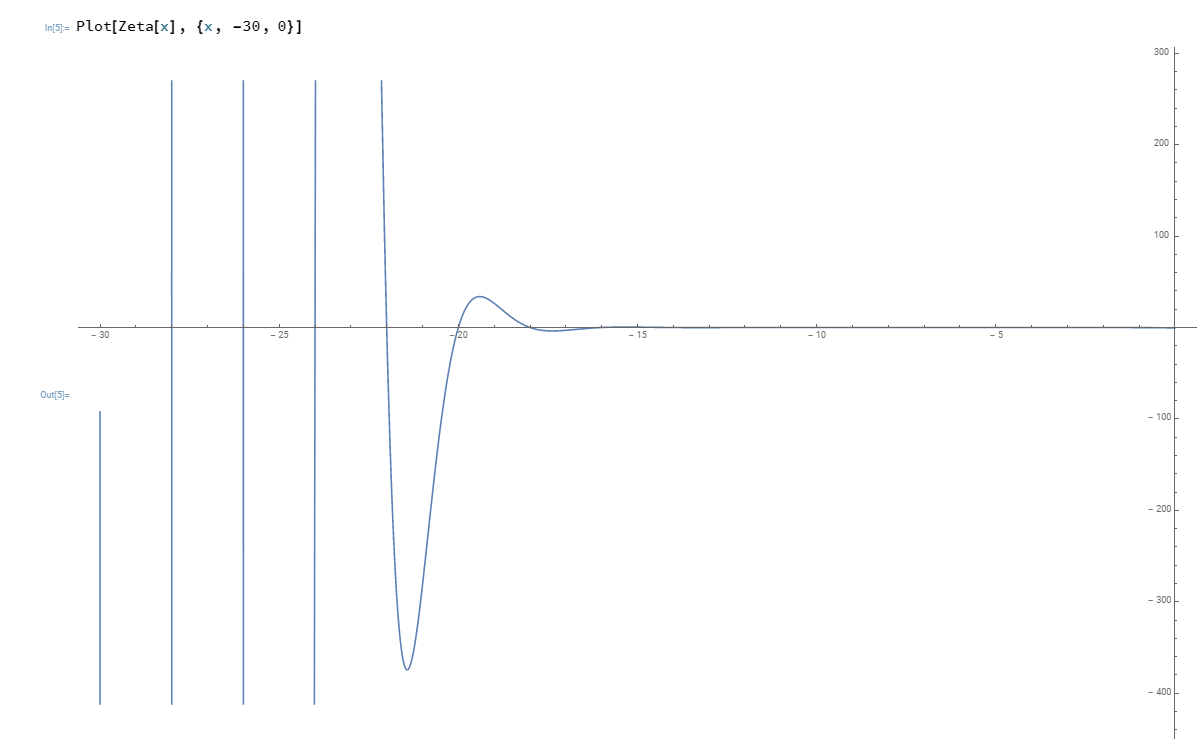
\includegraphics[width=\textwidth]{zeros.png}
  \begin{center}
  \caption{Graph of Euler-Riemann zeta function using
Wolfram|Alpha Open Code and built-in math functions.}
    \label{fig:zeros}
  \end{center}
  \end{figure}

In the graph above we can see how the Euler-Riemann zeta function intersects x-axis on negative
even integers. However, each time the absolute value of an argument increases, this feature of
Euler-Riemann zeta function will be discussed next. Also, we can ensure the values of Euler-
Riemann zeta function by using MATLAB as shown in Figure \ref{fig:zerosv}.

\begin{figure}[h!]
  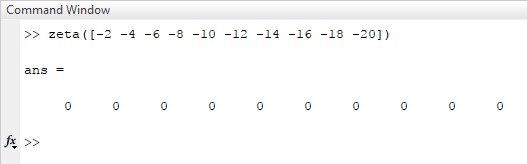
\includegraphics[width=\textwidth]{zerosv.png}
\begin{center}
  \caption{Euler-Riemann zeta
function values for
negative even integers,
calculated in MATLAB.}
  \label{fig:zerosv}
\end{center}
\end{figure}

\subsection{Negative Odd Arguments}

Secondly, as I discussed the “trivial zeros" for Euler-Riemann and as we have proved the product
form for Euler-Riemann function, now we can find the values for negative odd integers. We know
three ways of presenting Euler-Riemann zeta function:

\begin{equation}
  \zeta(s)=\prod_{p \text{ prime}}^{\infty} {(1-p^{-s})}^{-1}=\sum_{n=1}^{\infty} n^{-s}=2^s\pi^{s-1}\sin(\frac{\pi s}{2})\Gamma(1-s)\zeta(1-s)\\
  \end{equation}

By using the notations below and Euler's formula that we learned during our course of complex
numbers, we can see how they lead\cite{Bern} to the following formula
for negative integer arguments:

\begin{equation}
  \label{bnn}
  \zeta(1-n)=-\frac{B_n}{n} \text{, $n\in N$}\\
  \end{equation}

$B_n$ is the $n^{th}$ Bernoulli number. Bernoulli numbers are a series of rational numbers, which are
mainly used in number theoury. The values for nth value of Bernoulli numbers can defined in the
following equation\cite{BernSeq}, where for
every odd $n$, $B_n=0$:

\begin{equation*}
  B_n=\frac{\sum_{k=1}^{n} \sum_{j=1}^{k} \frac{(-1)^j (j^n \binom{1+n}{-j+k}) }{\binom{n}{k}} }{1+n}
  \end{equation*}

The table below shows the values for the first 10 even Bernoulli numbers' arguments. These values
have been calculated by using Wolfram|Alpha Open Code service. Table \ref{tab:bernoulli} will show
first 10 non-zero elements' values of Bernoulli numbers.

\begin{table}[h!]
  \begin{center}
    \begin{tabular}{c | c | c | c | c | c | c | c | c | c | c}
      $n$ & 0 & 1 & 2 & 4 & 6 & 8 & 10 & 12 & 14 & 16\\
      \hline
      $B_n$ & 1 & $-\frac{1}{2}$ & $\frac{1}{6}$ & $-\frac{1}{30}$
      & $\frac{1}{42}$ & $-\frac{1}{30}$ & $\frac{5}{66}$ & $-\frac{691}{2730}$
      & $\frac{7}{6}$ & $-\frac{3617}{510}$\\
    \end{tabular}
    \caption{First 10 Non-Zero Elements of Bernoulli Numbers}
    \label{tab:bernoulli}
  \end{center}
 \end{table}

Subsequently, we can now find finite values for Euler-Riemann zeta function with negative odd
integer arguments. Referring to the previous chapter with the series $1+2+3+4+5+...$, now
we can present the following series in the form of Euler-Riemann zeta function with Bernoulli
numbers and find a convergent value for the series.

\begin{equation}
  \sum_{n=1}^{\infty} n = 1+2+3+4+5+...=\zeta(-1)=\zeta(1-2)=-\frac{B_2}{2}=
  -\frac{\frac{1}{6}}{2}=-\frac{1}{12}\\
  \end{equation}

We can apply equation \ref{bnn} to any natural even number and by that forming a divergent series,
where it would be possible to find a value to which the series converges. As an example, I would like
to test out powers 3, 5 and 7:

\begin{align*}
  \sum_{n=1}^{\infty}n^3&=1^3+2^3+3^3+4^3+...=\zeta(-3)=\zeta(1-4)=
  -\frac{B_4}{4}=-\frac{-\frac{1}{30}}{4}&=&\frac{1}{120}\\
  \sum_{n=1}^{\infty}n^5&=1^5+2^5+3^5+4^5+...=\zeta(-5)=\zeta(1-6)=
  -\frac{B_6}{6}=-\frac{\frac{1}{42}}{6}&=-&\frac{1}{252}\\
  \sum_{n=1}^{\infty}n^7&=1^7+2^7+3^7+4^7+...=\zeta(-7)=\zeta(1-8)=
  -\frac{B_8}{8}=-\frac{-\frac{1}{30}}{8}&=&\frac{1}{240}\\
\end{align*}

\section{Conclusion}

In the conclusion, throughout this exploration, we have explored the methods of finding the limit
for divergent series. We should know that these limits are found using mathematical manipulations
with infinity, meaning that we assume that we have an infinite amount of integers and elements,
we should rather know that these convergent values have been found because we analytically
extended Euler-Riemann zeta function. People tend to think of these results as "mathematical
tricks" and theories to play around, however, these results are actively used in physics, as in physics we
can not have an infinity or indefinite results, results should be finite, precise and exact.
For example,
the limit of $\zeta(-1)$ is used the "String Theory" by Joseph Polchinski\cite{String} in order to compute energy
levels of a single string. Also, the series $1+2+3+4+...=-1/12$ has been mentioned in the media
by Numberphile in video – "ASTOUNDING: 1+2+3+4+5+...= -1/12".\cite{Numberphile} Sure, at the end we came
up with a rather extraordinary result, which makes Mathematics as a science beautiful and
encouraring for further researches and explorations.\\
I would like to end this exploration with an idea that relatively to its full potential, Mathematics is
quite young science, even if it may seem otherwise. From the very beginning of its existence, Mathematics
helped us and guided us through the mysteries and secrets of the world around us. People were working on
Mathematics by using their imagination, reasoning and emotions. So that Mathematics became a result
of humanity's thoughts and hope for the better future. We should never stop improving and working on
Mathematics, no matter how difficult or unsolvable the future challenges may seem.

%\newpage
\bibliography{cods}
\bibliographystyle{ieeetr}

\end{document}